\chapter{Modeling Legged Locomotion}
\label{sec:ModelingLeggedLocomotion}
\index{models of locomotion}

We develop models of locomotion in order to understand various aspects of the dynamics of the motion of locomotives. The objective of a model of locomotion is to describe the kinematic structure of legs (links, joints, supports, and actuators) and the nature of the loading on this structure or the energy transfer (e.g. impact loading, spring energy), in a manner that makes sense for a particular model, that can realistically represent the forces and motions that occur in actual locomotion. Accordingly, a model of locomotion includes illustrations of its kinematic structure and equations that describe force interactions or energy transfer that correspond to the behavior of the kinematic structure in a manner that makes sense for a particular model. We can compare some models to each other by using the metric of metabolic cost of transport\index{metabolic cost}. The description of the models is not strictly motivated by such goals though. At various points, some interesting expressions are developed for their own sake.

This chapter first presents the equations of motion in the notation of this text, and then describes three models of locomotion. In order of increasing complexity these are the point mass model, the collisional model, and the spring-loaded inverted pendulum (SLIP) model.

\section{Equations of Motion} %(notes page 40-43)
\label{sec:EquationsOfMotion}
\index{equations of motion}
\index{motion, equations of}

The fundamental equations of dynamics are provided here without derivation. Such derivations can be found in any introductory dynamics textbook. The equations here are presented to provide the notation and symbols that are used throughout the text, as well as to clarify the equations of motion for multi-object systems. The locomotion models in this text consist of only point masses, and so the rigid object formulation of the equations of motion is not presented.

The terms particle and point mass are used interchangeably. The vectors here are vectors in two dimensional space, as all of the models are two-dimensional. The vector $\vr$ denotes a position in space, the vector $\vv$ denotes the velocity of a position, and the vector $\va$ denotes the acceleration of a position. The center of mass of an object is denoted as $G$. The notation $G/C$ reads as ``the center of mass with respect to point C''. If a quantity is not denoted as being ``with respect to'' a point (e.g. $\vr_{i}$), then the point is assumed to be defined with respect to the origin of the system $O$.

\subsubsection*{A single point mass}
For a point mass\index{point mass}, the equations of motion are simple. Only linear momentum balance (LMB)\index{linear momentum balance} and energy balance are relevant, since a particle cannot rotate. The linear momentum of a particle is

\begin{equation}
\vL = m\vv
\end{equation}

Linear momentum balance, or Newton's second law, for a particle states that

\begin{align}
\sum_{i} \vF_{i} &= \vLdot \\
&= m \va
\end{align}

where $\vF_{i}$ is the $i$-th contact or body force acting on a particle with mass $m$. The sum of the vector forces gives rise to the particle's acceleration $\va$. The energy of a particle $E$, neglecting friction, is given by

\begin{align}
E &= \KE + \PE \\
&= \frac{1}{2}mv^{2} + mgh
\end{align}

\subsubsection*{Collection of point masses}
Most of the models in this text involve multiple point masses. For a system of point masses such as in the general example of figure \ref{fig:EnergyAccounting} the center of mass relative to an arbitrary point $C$ is

% FIGURE
\begin{figure}[h]		% h="here" t="top" b="bottom" p="separate page"
\begin{centering}
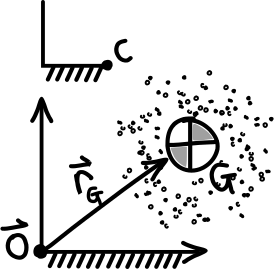
\includegraphics[width=0.3\textwidth]{Figures/EnergyAccounting}\par
\end{centering}
\caption[Diagram: Energy Accounting]{Energy accounting. This figure shows how to find the center of mass for a general system of point masses. The center of mass can be be described in any reference frame. [chris: why is this figure called Energy Accounting?]}
\label{fig:EnergyAccounting}
\end{figure}
%

\begin{equation}
\vr_{G/C} = \frac{\sum \vr_{i/C} m_{i}}{\sum m_{i}}
\label{eq:CenterOfMass1}
\end{equation}

Upon simple rearranging, equation \ref{eq:CenterOfMass1} yields 

\begin{equation}
m_{tot} \vr_{G/C} = \sum_{i} \vr_{i/C} m_{i}
\label{eq:CenterofMass2}
\end{equation}

where $m_{tot} = \sum m_{i}$. If equation \ref{eq:CenterOfMass1} is differentiated with respect to time, it relates the velocity of the system's center of mass to the velocities of the objects that compose the system. For a system of particles, the linear momentum is the sum of the linear momentum of each particle.

\begin{equation}
\vL = \sum_{i} m_{i} \vv_{i} = m_{tot} \vv_{G}
\end{equation}

Proceeding naturally, the linear momentum balance for a system of point masses

\begin{equation}
\sum_{i} \vF_{i}^{ext} = \vLdot
\end{equation}

Only external forces are relevant for LMB. Internal forces are defined as being between two masses within the system, and Newton's second law requires these forces to cancel each other. The external forces can arise from fields such as gravity, or contact with a surface or a mass that is not part of the system.

The angular momentum of the system with respect to a point $C$ is defined as

\begin{equation}
\vHC = \sum_{i} \vr_{i/C} \times m_{i} \vv_{i}
\end{equation}

For the purposes of this text, the point $C$ is fixed in space. This requirement allows the simplification of time derivatives of the angular momentum. The positions and velocities can be written relative to the center of mass of the system, yielding

\begin{equation}
\vHC = \sum_{i} (\vr_{i/G} + \vr_{G/C}) \times (\vv_{i/G} + \vv_{G/C}) m_{i}
\end{equation}

When the terms in this equation are expanded, the angular momentum is

\begin{align}
\vHC &= \sum_{i} \vr_{i/G} \times \vv_{i/G} m_{i} + \vr_{G/C} \times \vv_{G/C} \sum_{i} m_{i} \notag \\
& + \sum_{i} \vr_{i/G} m_{i} \times \vv_{G/C} + \vr_{G/C} \times \sum_{i} \vv_{i/G} m_{i}
\label{eq:AMBSystem}
\end{align}

Based on the definition of the center of mass, the summation $\sum \vr_{i/G}m_{i}$ and its derivatives are zero. As a result, the second two terms of equation \ref{eq:AMBSystem} are zero. The first term in the expansion is a sum of the angular momentum of each particle in the system with respect to the center of mass of the system. The second term is the angular momentum of the system's center of mass with respect to the arbitrary point $C$. Thus the angular momentum is concisely written as

\begin{equation}
\vHC = \vH_{/G} + \vH_{G/C}
\end{equation}

The utility of angular momentum expressions is primarily for understanding the behavior of a system after a collision. On the other hand, Angular momentum balance is used in general to solve for the time-dependent loading on or motion of a system. The quantity of interest for angular momentum balance (AMB) is the time rate of change of the angular momentum. 

\begin{align}
\vHdotC &= \sum_{i} \vr_{i/G} \times \va_{i/G} m_{i} + \vr_{G/C} \times m_{tot} \va_{G} \\
 &= \vHdot_{/G} + \vHdot_{G/C} 
\end{align}

The differentiation actually yields two other terms as a result of the product rule of differentiation, but those terms vanish because $\vv_{i} \times \vv_{i} = 0$. AMB, provided in equation \ref{eq:AMB}, is expressed similarly to LMB.

\begin{equation}
\sum_{i} \vM_{/C}^{ext} = \vHdotC
\label{eq:AMB}
\end{equation}

The kinetic energy of a system of point masses is

\begin{equation}
\KE = \frac{1}{2} \sum_{i} m_{i} (\vv_{i} \cdot \vv_{i})
\end{equation}

The kinetic energy can be split into (1) the kinetic energy of all the point masses in the system with respect to the center of mass of the system, and (2) the kinetic energy of the center of mass of the system. Logically, a collection of particles that are in circular orbit around a fixed center of mass still has kinetic energy even though its center of mass is not moving. If the velocity is written as with respect to the center of mass of the system, the kinetic energy is expressed as

\begin{equation}
\KE = \frac{1}{2} \sum_{i} m_{i} (\vv_{G} + \vv_{i/G}) \cdot (\vv_{G} + \vv_{i/G})
\label{eq:CollectionKE2}
\end{equation}

One of the terms in the expansion of equation \ref{eq:CollectionKE2} vanishes because of the defintion of the center of mass. This yields

\begin{align}
\KE &= \frac{1}{2} \sum_{i} m_{i} v_{i/G}^2 + \frac{1}{2} m_{tot} v_{G}^2 \\
&= \KE_{/G} + \KE_{G}
\label{eq:Konig}
\end{align}

$\KE_{/G}$ denotes the ``relative'' kinetic energy, and $\KE_{G}$ denotes the ``center of mass'' kinetic energy. equation \ref{eq:Konig}, is known as Konig's theorem (also seen as K\"{o}nig or Koenig).

\section{The Point Mass Model} %(notes page 9-12)
\label{sec:ThePointMassModel}
\index{models of locomotion!point mass}

\begin{quote}

\emph{``A wealthy playboy is disappointed with his stable of racehorses. He hires an economist, a biologist, and a mathematician to advise him how to develop a winning racehorse. The economist devises a system of incentives to motivate the horses to produce optimal speed. After several horses die of starvation, the playboy fires the economist. He fires the biologist after being told that he will have an award winning racehorse in only 200 generations of careful breeding. Finally, the playboy asks the mathematician if he has solved the problem. The mathematician excitedly answers that after much deep thought he has worked out a beautiful solution: First assume the horse is a sphere...''}

\end{quote}

One way to model locomotion is by assuming the entire body is a point mass. This is a useful way to model a human because this assumption greatly reduces the complexity of the equations of motion needed to describe human locomotion. The model may also be accurate to a certain degree; a human's legs account for about only 44\% of the mass of the body \cite{winter92}\todo{Chris: 44\% doesn't sound too low} . We focus only on simple and abstract expressions for the energy interactions of the motion, as the motion itself is basic. \todo{Alan: this last sentence could use some clarification} 

A human can be reduced to a point mass as shown in figure \ref{fig:PersonFBD} if the complex operation of muscles, arms, and legs are neglected. In this free body diagram, the weight of the human acts at its center of mass, the rest of the body is massless, and both friction and normal forces may act at its feet in the appropriate directions. Additionally, forces such as drag can counter forward motion, and such forces act at the center of mass of the human. 

% FIGURE
\begin{figure}[h]		% h="here" t="top" b="bottom" p="separate page"
\begin{centering}
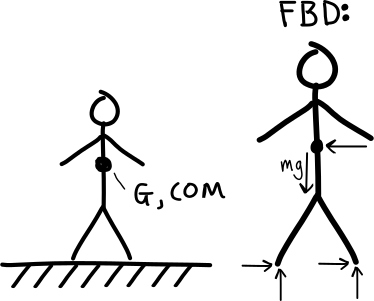
\includegraphics[width=0.4\textwidth]{Figures/PersonFBD}\par
\end{centering}
\caption[Diagram: Free Body Diagram of a Human]{Free body diagram of a human. For the point mass model of a human, the human is reduced to a single point mass located at its center of mass. The force of gravity acts at the center of mass, as well as air drag if it is included. The force of friction and the normal ground reaction act at the human's massless feet. Of course, internal forces do not appear in the free body diagram.\todo[inline]{Alan: I am not sure if that horizontal vector was meant to model drag or not when I drew this... I'm just hoping it wasn't for something that I'm forgetting right now. }}
\label{fig:PersonFBD}
\end{figure}
%

Although walking appears to be a smooth process, it can actually be viewed as a series of collisions. The collisional nature of this point mass motion is illustrated in figure \ref{fig:Bounce}. In essence, the point mass model of a human is a bouncing particle. The particle does not collide directly with the ground, but collides through massless legs. The objective here is to find a relation between the work $W$ performed by the locomotive and the metabolic energy cost $E_{m}$\index{metabolic cost} of providing that work \cite{ruina05}. This work is performed by the locomotive's muscles to overcome the collision of the point mass in each stride. Positive work denotes work done \emph{by} the muscles on the skeleton.

The stride, or gait cycle, is divided into a falling portion that occurs before the collision of the mass with the ground, and a rising portion after the collision. The collision provides an impulsive vertical upward force that results in a new vertical velocity of the mass. If drag is neglected, there are no forces in the horizontal direction and the locomotive travels at a constant horizontal speed.

The minus sign and positive sign in figure \ref{fig:Bounce} denote the motion before and after the collision. Before the collision, the leg muscles are in \emph{eccentric}\index{contraction!eccentric} contraction, which means they are elongating under tension. In this ``contraction'', the muscles are performing negative work on the body. After the collision, the leg muscles are in \emph{concentric}\index{contraction!concentric} contraction, which means they are shortening and doing positive work on the body.

% FIGURE
\begin{figure}[h]		% h="here" t="top" b="bottom" p="separate page"
\begin{centering}
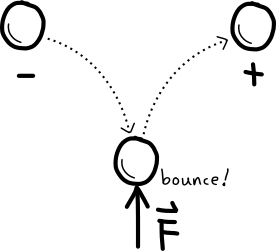
\includegraphics[width=0.3\textwidth]{Figures/Bounce}\par
\end{centering}
\caption[Diagram: Point Mass Model of Human Locomotion]{Point mass model of human locomotion. The human is a single point mass that periodically collides with the ground. The legs of the human are ignored so that the ground reaction is a single vertical force that helps redirect the velocity of the human. The minus sign and positive sign denote the motion before and after the collision.}
\label{fig:Bounce}
\end{figure}
%

Since we desire a relationship between energy (metabolic cost) and total work (muscle work) over a single stride, we apply the work-enegy theorem to this model over a single stride.

\begin{align}
P &= \vF \cdot \vv \notag \\
W &= \int \vF \cdot d\vr \notag \\
  &= E^{+}_{K} - E^{-}_{K} \notag \\
 &= \Delta E_K
\label{eq:CollisionalWork}
\end{align}
\index{collisional work}

where $E_{K}$ is the kinetic energy of the mass, $E_{K}^{+}$ is its kinetic energy after the collision, and $E_{K}^{-}$ is its kinetic energy before the collision. If we consider steady locomotion on level ground, then the motion is periodic and the kinetic energy does not change from stride to stride. By equation \ref{eq:CollisionalWork}, the net work from stride to stride must be zero as well. If the muscle work in a stride is divided into positive and negative portions as described above, then

\begin{equation}
W = W_{pos} + W_{neg} \approx 0
\label{eq:CollisionalWork2}
\end{equation}

equation \ref{eq:CollisionalWork2} is not an equality because some work goes into nonconservative energy dissipation, such as the deformation of parts of the body that are not muscle.

\todo[inline]{Alan: a general note on the use of "metabolic." The net-zero work concept makes sense if you're thinking only of work in the traditional energetics sense of the word. I feel like many people to whom this whole subject may be new would have trouble with the net-zero work concept because they may think "oh, well then why do I get tired, need to eat, etc. after walking with a steady periodic motion?" The answer is because the way muscles work, you still consume calories to do the negative work. It's not like we're getting energy back by falling. The next section explains this well, with the "b1" and "b2" constants, but the lead-in may be a little confusing. I don't know if this should be made explicit or not.}

We are now equipped to relate muscle work to metabolic energy cost. Recalling figure \ref{fig:MetabolicCost}, the metabolic cost can be expressed as

\begin{displaymath}
   E_{m} = \left\{
     \begin{array}{lr}
       b_{1} W & : W \geq 0\\
       b_{2} |W| & : W < 0
     \end{array}
   \right.
\end{displaymath}

where $E_{m}$ is always positive, $W$ is muscle work, $b_{1}$ is an empirical conversion factor for negative muscle work (as with the eccentric contraction), and $b_{2}$ is an empirical conversion factor for positive muscle work (as with the concentric contraction). The metabolic cost of one stride is then:

\begin{align}
E_{m} &= b_{1} W_{pos} + b_{2} |W_{neg}| \\
&\approx (b_{1} + b_{2})W_{pos}
\end{align}

Collecting in terms of $W_{pos}$ is possible because of the principles used to make the approximation in equation \ref{eq:CollisionalWork2}. If $W_{pos}$ is nearly equal to $|W_{neg}|$, one can be substituted for the other and the sum of the empirical constants $b = b_{1} + b_{2}$ may then be collected as one expression. Figure \ref{fig:MetabolicCost} indicates that $b_{1}\approx4$ and $b_{2}\approx1$. This means that the caloric energy spent by the body while walking is approximately 5 times the positive work required to move the body. 

\todo[inline]{[chris: can we quantify how much energy this actually is? I can use the discussion of muscles in section \ref{sec:IntroductionToMuscles}, or could refer the reader to employ methods provided in section \ref{sec:OptimizationInLocomotion}] \\ Alan: I think the best we can do is to refer people to section \ref{sec:OptimizationInLocomotion}. That deals with the integration along the path, which is really the only way to quantify the energy used (by the model).}

The trajectory traced by the center of mass in our point mass model shows that the motion is not smooth. This conflicts with our own perception of our motion as being a smooth process. The point mass motion is better applied to the motion of a hopping frog. This ``gait" is described by figure \ref{fig:HoppingFrogModel}. The definition for the cost of transport (COT) is easily applied here to provide 

\begin{equation}
COT = \frac{E_{m}}{mgd} = \frac{bW_{pos}}{mgd}
\end{equation}

For more detail about the hopping frog model, see Rashevsky 1948 \cite{rashevsky48}.

% FIGURE
\begin{figure}[h]		% h="here" t="top" b="bottom" p="separate page"
\begin{centering}
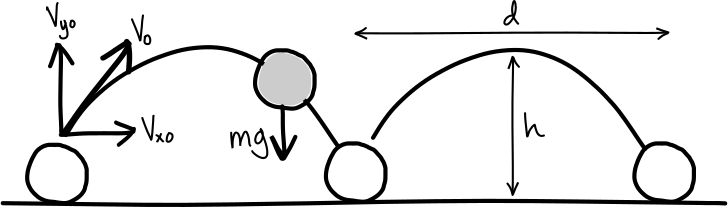
\includegraphics[width=0.8\textwidth]{Figures/HoppingFrogModel}\par
\end{centering}
\caption[Diagram: Hopping Frog Model]{Hopping frog model. The point mass model applies better to the motion of a hopping frog. This motion is characterized by two parameters: a jump distance $d$ and height $h$ of the hops.}
\label{fig:HoppingFrogModel}
\end{figure}
%

However, most animals continue traveling throughout this collision. In fact, the kinetic energy of a locomotive typically remains constant through steady motion \cite{ruina05}). Additionally, the up and down motion traced by the center of mass is usually much smaller than the forward motion. In terms of figure \ref{fig:HoppingFrogModel}, this means that the change in $h$ throughout a gait cycle is much smaller than $d$. For these reasons, we explore a more detailed model of the legs' trajectory and the forces upon the body from the ground.

\todo[inline]{Alan: the hopping frog model stuff either needs to be cut out, or explained better in a way that makes it clear why it's even here.}

\begin{comment}
For conservation of energy, the positive muscle work must be the same as the net mechanical energy lost in one stride \cite{ruina05}. 
\end{comment}

\section{The Collisional Model} % (notes page 12-19)
\label{sec:TheCollisionalModel}
\index{models of locomotion!collisional}

We developed the point mass model under the claim that legs can be ignored since the mass of legs is often significantly less than that of the whole body. However, legs are useful for accurately describing the collision of the body with the ground.

%[chris]: how do we deal with one leg at a time?

This model incorporates, initially, a single massless leg to allow for a more detailed force interaction \cite{ruina05}. A simple illustration of the collisional model is given in figure \ref{fig:LegDiagram}. The collision does not occur at a single point but over a contact region $W$ in between the falling and rising portions of the stride. Instead of a directly upward force upon the point mass from the ground collision, the force on the point mass is conveyed through the locomotive's legs throughout the entire contact region. The leg only conveys a force in compression, and there are no moments generated by the collision (e.g. a hip torque). Although the collision occurs over a distance, the collision still occurs quickly ($\Delta t \rightarrow 0$). As a result, the force associated with the impact dominates non-collision forces such as weight.

% FIGURE
\begin{figure}[h]		% h="here" t="top" b="bottom" p="separate page"
\begin{centering}
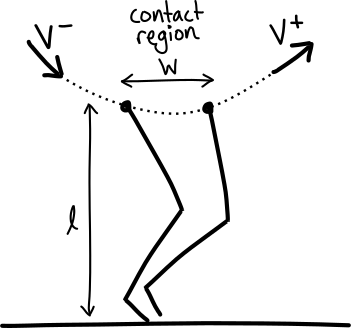
\includegraphics[width=0.4\textwidth]{Figures/LegDiagram}\par
\end{centering}
\caption[Diagram: Legs in the Collisional Model]{Legs in the collisional model. The impact of the ground on the locomotive is conveyed through massless legs. The impact occurs over a contact region $w$, which is the horizontal distance that the locomotive moves while (one of) its legs are in contact with the ground. The speed before the contact is $v^{-}$ and the speed after the collision is $v^{+}$. During the contact, the distance between the center of mass of the locomotive and the ground is approximated as $l$.}
\label{fig:LegDiagram}
\end{figure}
%

If we approximate that $W \ll l$, then the angle of the force $F$ is constant throughout the collision. In figure \ref{fig:CollisionDiagram}, the angle of the force is given by the unit vector $\hat{\lambda}$. The velocity of the point mass before and after the collision is given by $\mathbf{v}^{-}$ and $\mathbf{v}^{+}$, respectively. The collision causes a net deflection $\phi \ll 1$, which can be decomposed into components

\begin{equation}
\phi = \phi^{-} + \phi^{+}
\label{eq:PhiDecompose}
\end{equation}

that describe the direction of the initial and final velocities relative to the line given by $\hat{t}$.

%[chris]: is the rest of the mass, from waist up, considered to be a point mass?

% FIGURE
\begin{figure}[h]		% h="here" t="top" b="bottom" p="separate page"
\begin{centering}
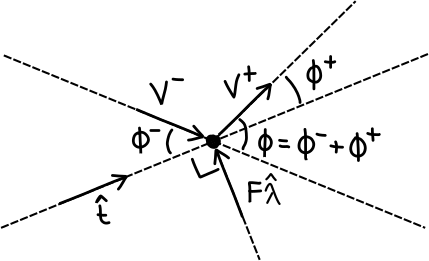
\includegraphics[width=0.5\textwidth]{Figures/CollisionDiagram}\par
\end{centering}
\caption[Diagram: Collisional Model Impulse]{Collisional model impulse. This diagram describes the change in velocity (direction and magnitude) that occurs during the collision of the leg with the ground. The contact $w$ is assumed to be small, but this diagram is ``located'' at the center of mass throughout the collision. The direction is constant in the direction of $\ul$. The unit vector $\ut$ is defined as perpendicular to $\ul$. The incoming deflection of the velocity is the angle $\phi^{-}$ between $v^{-}$ and $\ut$. The outgoing deflection of the velocity is the angle $\phi^{+}$ between $v^{+}$ and $\ut$.}
\label{fig:CollisionDiagram}
\end{figure}
%

\subsubsection*{Kinetic energy and the collision}

Collisions are classically viewed as dissipative interactions. In this case however, the muscular mechanisms involved in the collisions can even permit the interaction to increase the kinetic energy of the locomotive. We decompose the velocity of the point mass into components as $\mathbf{v} = v_{\lambda} \ul + v_{t} \hat{\mathbf{t}}$ so that we can write the kinetic energy of the mass as in equations \ref{eq:CollisionsKE}.

\begin{equation}
E_{K} = E = \frac{1}{2}m(v_{\lambda}^{2} + v_{t}^{2})
\label{eq:CollisionsKE}
\end{equation}

In this section, the kinetic energy is written as $E$ for clarity. The change in kinetic energy as a result of the collision is then $\Delta E = E^{+} - E^{-}$, where

\begin{align}
E^{-} &= \frac{1}{2}m[(v_{\lambda}^{-})^2 + (v_{t}^{-})^2]  \notag \\   
E^{+} &= \frac{1}{2}m[(v_{\lambda}^{+})^2 + (v_{t}^{+})^2] \notag
\end{align}

We can simplify these energy terms using the assumptions we have made. During the collision, no forces act in the $\hat{t}$ direction, so $v_{t}^{+} = v_{t}^{-}$. Since $\phi$ is small, $\sin{\phi} \approx \phi$ and so the velocity in the direction of $\hat{\lambda}$ before and after the collision is simply $v_{\lambda}^{-} = -v \phi^{-}$ and $v_{\lambda}^{+} = v \phi^{+}$.

% FIGURE
\begin{figure}[h]		% h="here" t="top" b="bottom" p="separate page"
\begin{centering}
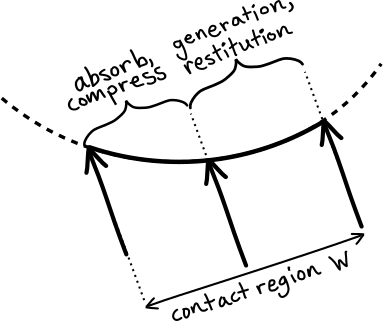
\includegraphics[width=0.4\textwidth]{Figures/BounceEnergy}\par
\end{centering}
\caption[Diagram: Energy in the Collisional Model]{Energy in the collisional model. The collision is divided into two portions: In the initial absorption portion, kinetic energy $E_{a}$ is absorbed (not all lost though) while the human approaches the ground. In the subsequent generation portion, the human generates and recovers kinetic energy in the quantity $E_{g}$ while starting to rise.}
\label{fig:BounceEnergy}
\end{figure}
%

The collision can be divided into two portions as in figure \ref{fig:BounceEnergy}, an absorption/compression portion and a generation/restitution portion, The change in kinetic energy across the collision can be written in terms of these portions of the collisions.

\begin{align}
\Delta E^{*} &= E_{g} - E_{a} \notag \\
  &= \frac{1}{2} m v^{2} \displaystyle\left[ (\phi^{+})^{2} - (\phi^{-})^{2} \displaystyle\right] \notag \\
 &= mv^{2} \left( \frac{\phi^2}{2} - \phi \phi^{-} \right)
\label{eq:GenerateAbsorbKE}
\end{align}

where $E_{a}$ is the absorbed energy and $E_{g}$ is the generated energy in the collision, the $v_{t}$ terms drop out, and equation \ref{eq:GenerateAbsorbKE} has made use of equation \ref{eq:PhiDecompose}. It is important to understand that this is the change in kinetic energy over just the collision, not over the entire gait cycle. For this reason, the change in kinetic energy is designated with a superscript asterisk. This distinction will be important when expressing the metabolic cost of locomotion later in this section. equation \ref{eq:GenerateAbsorbKE} has been written in its apparently contrived form to bridge it to an expression that employs impulse.

% FIGURE
\begin{figure}[h]		% h="here" t="top" b="bottom" p="separate page"
\begin{centering}
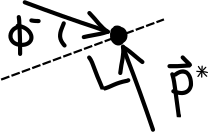
\includegraphics[width=0.18\textwidth]{Figures/Impulse}\par
\end{centering}
\caption[Diagram: Impulse in the Collisional Model]{Impulse in the collisional model. The impulse acts along the direction of the impact force $\ul$.}
\label{fig:Impulse}
\end{figure}
%

The impulse delivered to the point mass is $\mathbf{P}^{*} = P^{*}\hat{\lambda}$, as shown in figure \ref{fig:Impulse}. Using our approximations for velocity, the impulse is

\begin{align}
\vec{\mathbf{P}}^* &= mv(\phi^{+} - (-\phi^{-}))\ul\\
P^* &= mv\phi
\label{eq:CollisionImpulse}
\end{align}

Using this impulse, the two terms in equation \ref{eq:GenerateAbsorbKE} become

\begin{equation}
\Delta E^{*} = \frac{ (P^{*})^{2}}{2m} + \vec{\mathbf{P}}^{*} \cdot \vec{\mathbf{v}}^{-}
\label{eq:GAKE2}
\end{equation}

Equation \ref{eq:GAKE2} can be most easily understood by expressing its second term as equation \ref{eq:GenerateAbsorbIntermediate2} to arrive back at equation \ref{eq:GenerateAbsorbKE}.

\begin{align}
\vec{\mathbf{v}}^{-} &= v(-\phi^{-} \ul + 1\hat{\mathbf{t}}) \label{eq:GenerateAbsorbIntermediate1} \\
(P^{*} \ul) \cdot \vec{\mathbf{v}}^{-} &= (mv\phi)(-v\phi^{-})(\ul \cdot \ul) \label{eq:GenerateAbsorbIntermediate2}
\end{align}

where the small angle approximation $\cos{\phi} \approx 1$ has been made. In general, $\Delta E^{*}$ can be either positive or negative. \todo[inline]{chris: we don't use this form of delta E, so should we include it?}

Typically, the change in velocity of colliding masses is described by a \textit{coefficient of restitution} $e_{r}$, which is the relative speed of separation divided by the relative speed of approach of two colliding masses. This quantity is useful because it describes how elastic a collision is.

\begin{displaymath}
   e_{r} = \left\{
     \begin{array}{lr}
       1 & : \mbox{perfectly elastic}\\
       0 & : \mbox{perfectly plastic}
     \end{array}
   \right.
\end{displaymath}

For the collisional model, this coefficient is 
\begin{displaymath}
e_{r} = \frac{|v_{\lambda}^{+}|}{|v_{\lambda}^{-}|} = \frac{\phi^{+}}{\phi^{-}}
\end{displaymath}

However, this coefficient is not so useful for the scenario in which $\phi^{-} = 0$. This would be a ``collision'' that is not elastic, but actually ``generative'', such as jumping. Remember, the collision here is not necessarily strictly dissipative. For this reason we define a \textit{coefficient of generation} $e_{g}$. \index{coefficient of generation} \index{generation!coefficient of}

\begin{align}
e_{g} &= \frac{\mbox{[relative speed of separation] - [relative speed of approach]}}{\mbox{[relative speed of separation] + [relative speed of approach]}} \notag \\
&= \frac{\phi^{+} - \phi^{-}}{\phi^{+} + \phi^{-}}
\label{eq:CoefficientOfGeneration}
\end{align}

This cofficient has the properties:

\begin{displaymath}
   e_{g} = \left\{
     \begin{array}{ll}
     	1 & : \mbox{solely generative}, e_{r} = \infty\\
        0 & : \mbox{perfectly elastic}, e_{r} = 1\\
       -1 & : \mbox{perfectly plastic}, e_{r} = 0\\
     \end{array}
   \right.
\end{displaymath}

With some algebra,  $e_{g}$ for the collisional model can be expressed as 

\begin{displaymath}
e_{g}=\frac{\Delta E^{*}}{mv^{2}\phi^{2}/2}
\end{displaymath}

This is the ratio of the energy gained in the collision to the amount of energy that \emph{would} be in absorbed in a fully plastic collision with the same $v$ and $\phi$ \cite{ruina05}. This also yields another formula for the change in kinetic energy across the collision

\begin{equation}
\Delta E^{*} = e_{g} \frac{mv^{2} \phi^{2}}{2}
\label{eq:GenerateAbsorbKE3}
\end{equation}

We now endeavor to find the metabolic cost of locomotion for this collisional model, where the metabolic cost $E_{m} = b[\mbox{positive muscle work}]$. The quantity $b$ resembles an inverse efficiency, akin to a coefficient of performance from thermodynamics, and takes on a value between 4 and 5 for muscles and between 1.2 to 2 for motors. The \textit{elastic recovery coefficient} \index{elastic recovery coefficient} \index{coefficient!elastic recovery} $r$ is the fraction of absorbed energy $E_{a}$ that has been usefully or elastically stored and is thus available for muscle work as $E_{g}$, and $1-r$ is the fraction of absorbed energy that has been lost. This coefficient allows us to write

\begin{align}
\mbox{Positive generated muscle work} &= E_{g} - rE_{a} \\
\mbox{Absorbed energy that is lost} &= E_{a}(1-r)
\label{eq:ElasticRecovery}
\end{align}

The absorbed energy can be lost by general dissipation, or by negative muscle work that is not stored elastically.

\subsubsection*{Metabolic cost}

We now seek to determine the metabolic cost of locomotion using the collisional model. The collision occurs during only a small portion of the gait cycle. In general, energy interactions must occur during the other portions of the gait to maintain conservation of energy. Thus, the metabolic cost here is an \textit{inferred} metabolic cost \index{metabolic cost!inferred} because we assume that the minimum amount of positive work is performed throughout the remainder of the gait cycle. That is, the amount of positive work performed is only as much positive work as is required to recover from dissipation or energy loss in the collision. Basically, the locomotive is not kicking its feet between collisions.

We can express the metabolic cost in terms of $E_{a}$, $E_{g}$, and $r$. The use of an \textit{inferred} cost requires the examination of two different cases.

\begin{itemize}
\item \textbf{Dissipative collision}: $e_{g} \leq 0$, $\Delta E^* \leq 0$, $E_{g} \leq E_{a}$. Energy is lost over the course of the collision. To conserve energy, at least $E_a - rE_a$ positive work must be performed during the gait (outside of the collision). By using this quantity as the minimum positive work performed,

\begin{align}
E_{m}& = bE_{a}(1-r) \notag \\
 &= b\left(\frac{m v^{2} \phi^{2}}{8}\right)(1-r)(1-e_{g})^2
\label{eq:MetabolicCostCollisionalNeg}
\end{align}

For a perfectly plastic collision, $e_g$ = -1, with no energy recovery from muscles, $r$ = 0, $E_{m} = b E_{a}$.

\item \textbf{Generative collision}: $e_{g} \geq 0$, $\Delta E^* \geq 0$, $E_{g} \geq E_{a}$. Energy is gained over the course of the collision. Thus, the positive work performed throughout the gait must be at least the positive work performed during the collision.

\begin{align}
E_{m} &= b(E_{g} - r E_{a}) \notag \\
 &= b\left(\frac{m v^{2} \phi^{2}}{8}\right)\left[(1-r)(1-e_{g})^2 + 4e_{g}\right]
\label{eq:MetabolicCostCollisionalPos}
\end{align}

For a solely generative collision or jump from rest, $e_{g}$ = 1, with no energy recovery, $E_{m} = b \phi^2 v^2 m / 2$.
\end{itemize}

Again, the first case corresponds to a net energy loss during the collision, and a net energy gain during the remainder of the gait. The second case corresponds to a net energy gain during the collision, but a net energy loss during the remainder of the gait. In this formulation, it is assumed that the kinematic parameters $v$ and $\phi$ are known. The coefficients $e_{g}$ and $r$ could be obtained experimentally. The derivation of equations \ref{eq:MetabolicCostCollisionalNeg} and \ref{eq:MetabolicCostCollisionalPos} is left to the reader. A valuable result from these formulas is that a pseudo-elastic \index{pseudo-elastic} collision has a quarter of the metabolic cost of a fully plastic (absorbing) collision. A pseudo-elastic collision is just like a perfectly elastic collision in that the kinetic energy before and after the collision is the same (alas, $e_{g} = 0$) except that some energy $is$ dissipated in the collision but is replaced by additional muscle work. However, this is not apparent from the kinematics.

\subsubsection*{No-cost locomotion and multiple collisions}

Is it possible to achieve locomotion at no energy cost? \todo[inline]{chris: include why this would be neat} Logically, it is valuable to explore ways for a locomotive to minimize its $COT$. Remember that we have assumed that the cost of locomotion mostly comes from collisions. Then a model of locomotion in which collisions do not occur could potentially exhibit a very low $COT$. This question can be explored by examining \textit{brachiation}\index{brachiation}, which is the motion of swinging between overhead supports. This motion is exhibited by gibbon apes and by children on monkey bars. The kinematics of this motion is described in figure \ref{fig:Brachiation}. The locomotive's path alternates between pendular when swinging on a tree branch, and parabolic when in free flight subject to gravity \cite{bertram99}.

% FIGURE
\begin{figure}[h]		% h="here" t="top" b="bottom" p="separate page"
\begin{centering}
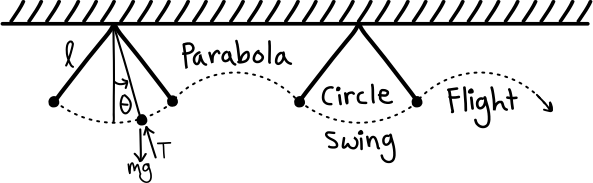
\includegraphics[width=0.7\textwidth]{Figures/Brachiation}\par
\end{centering}
\caption[Diagram: Brachiation]{Brachiation. Brachiation is the motion of swinging between overhead supports, as apes oft do. The motion consists of pendular swinging and a free flight. If the path of the motion is smooth, there is no collision and the motion is conservative.}
\label{fig:Brachiation}
\end{figure}
%
If the intersection of the parabola and circular arc is smooth (the direction of velocity is continuous), then no collision is required to redirect the locomotive's velocity from down to up. If no collision occurs, then the locomotion has no energy cost (neglecting friction). This model can be adapted to locomotion on the ground, since the model is analagous to upside-down running \cite{ruina05}. This can be done if the tension in the pendular motion is replaced with compression.

% FIGURE
\begin{figure}[h]		% h="here" t="top" b="bottom" p="separate page"
\begin{centering}
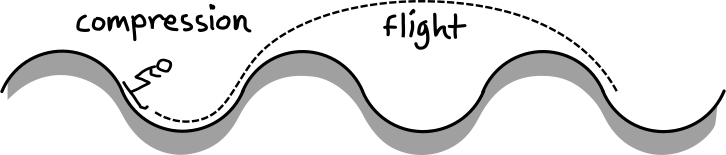
\includegraphics[width=0.7\textwidth]{Figures/Moguls}\par
\end{centering}
\caption[Diagram: Ski Slope Moguls]{Ski slope moguls. An analogue to brachiation is skiing on moguls, or small snow hills. The motion consists of a smooth path that alternates between ``compression'' and free flight.}
\label{fig:Moguls}
\end{figure}
%

A situation in which the pendular motion is characterized by compression is with skiing across snow moguls, as in figure \ref{fig:Moguls}. While in the trough between moguls, a skiier's velocity is redirected by a centripetal ``compressive" normal force. The skiier leaves the trough with a velocity that is parallel to the slope of the mogul at the point of departure. If the skiier enters the next trough with a velocity parallel to the mogul at the point of contact, then the velocity is continuous and no collision has occurred. In other words, no collision plane can be defined.

However, we have only moved the brachiation to the ground, and skiing is still very different from walking. A modified collisional model can resemble brachiation. In this modified collisional model, the locomotive experiences multiple collisions with the ground contact in each gait cycle rather than a single collision.

% FIGURE
\begin{figure}[h]		% h="here" t="top" b="bottom" p="separate page"
\begin{centering}
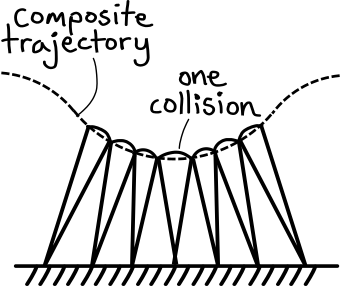
\includegraphics[width=0.3\textwidth]{Figures/MultipleCollisions}\par
\end{centering}
\caption[Diagram: Multiple collisions in the Collisional Model]{Multiple collisions in the collisional model. The collisional model is modified so that there are $n$ collisions per step, each conceivably executed by a different leg. The cost of locomotion is reduced by a factor of $n$ as compared to that for a one-legged locomotive.}
\label{fig:MultipleCollisions}
\end{figure}
%
\todo[inline]{chris: i think this entire chapter needs to be much clearer about what we're modeling. is it humans or what?}

Consider $n$ collisions that deflect the velocity of the locomotive by $\phi/n$, where $\phi$ is the total deflection from the $n$ collisions that is equivalent to the deflection $\phi$ from the single-collision model (figure \ref{fig:MultipleCollisions}). In this figure, it can be assumed that these $n$ collisions are executed by an $n$-legged locomotive and that each collision is performed by a different leg; the model is an abstraction from real scenarios. The parameters $v$, $e_{g}$ and $r$ are not changed in the $n$-collision model. Since the change in energy $\Delta E^*$ from a single collision is proportional to $\phi^2$, the metabolic cost for a single collision is reduced by a factor of $n^2$. Since these lower-cost collisions occur $n$ times, the \emph{total} cost of locomotion is reduced by a factor of $1/n$. As $n \rightarrow \infty$, the metabolic cost goes to zero.

This generalization allows the consideration of a number of gaits that describe at least two legs in the gait cycle. \todo[inline]{chris: gaits are discussed fundamentally in Optimization of Locomotion - Choosing a gait. should that be moved here? Alan: I think the section you're referring to is appropriate where it is, because it's discussing the choice in the context of optimization.} Four biped (two-legged) gaits are considered, as labeled (1) through (4) in the \textit{hodograph}\index{hodograph} in figure \ref{fig:Hodograph}. The hodograph contains plots of the velocity vector of the point mass as it evolves over the course of the collision. The full vector is only drawn in its initial and final positions, but the vector traces the dotted line path for the gait considered. The vector is plotted as always starting from the same location to depict how its magnitude changes as its direction changes by the full deflection $\phi$. The locomotive is indeed moving forward through the collision, though this is not apparent in the figure. The first of the two collisions is performed by a leg from a previous stance, and the second collision by a leg entering a new stance. Remember that velocity corresponds to a certain amount of kinetic energy, and for steady periodic motion the kinetic energy at the start of each gait cycle must be the same. Thus, the length of $v^{-}$ must be the same in every gait cycle. If negligible work is done during other portions of the gait, then the length of $v^{+}$ must be the same as the length of $v^{-}$. 

% FIGURE
\begin{figure}[h]		% h="here" t="top" b="bottom" p="separate page"
\begin{centering}
\subfloat[hodograph]{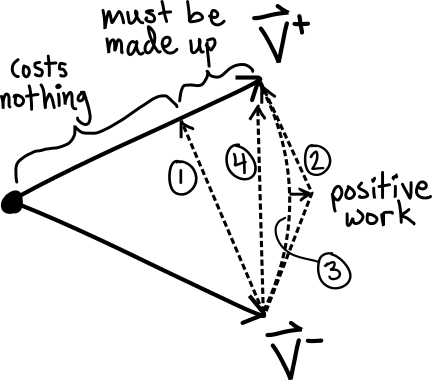
\includegraphics[width=0.3\textwidth]{Figures/Hodograph}\label{fig:Hodograph}}
\subfloat[incoming and outgoing impulses]{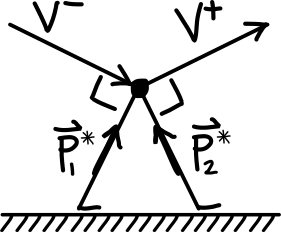
\includegraphics[width=0.3\textwidth]{Figures/StepTransition}\label{fig:StepTransition}}
\subfloat[simultaneous impulse force time history (for case 4)]{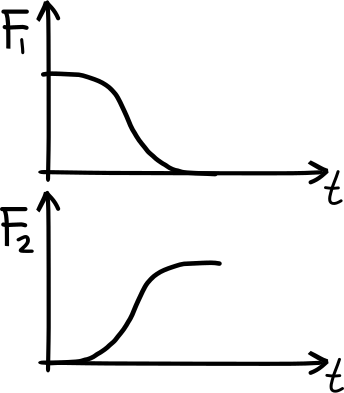
\includegraphics[width=0.3\textwidth]{Figures/ForcesFollowCircle}\label{fig:ForcesFollowCircle}}
\end{centering}
\caption[Diagram and Figure: Two-Collision Gaits in the Collisional Model]{Two-collision gaits in the collisional model. The hodograph (a) describes the four two-collision gaits explored in this section. A hodograph describes how a vector changes in both magnitude and direction by plotting the vector from the same point. The next diagram (b) shows the two impulses that belong to the first and second collisions that appear in some of the four gaits: the first impulse is perpendicular to the incoming velocity, and the second impulse is perpendicular to the outgoing velocity. The plots in (c) describe for case 4 the time history of the simultaneous forces that correpsond to the incoming and outgoing impulses. \todo[inline]{chris: subfigure captions need formatting}}
\label{fig:Ncollisional}
\end{figure}
%

\begin{itemize}
\item \textbf{Case 1, Fully plastic:} If the first impulse (collision) in figure \ref{fig:StepTransition} is taken away, then only the second impulse remains. This second instantaneous impulse removes the velocity along the direction of impact, and so this collision is purely plastic. The collision is termed ``passive" because no msucle work is performed during the collision. It is for this reason that this is the only case in which $v_{+}$ is not the same length of $v_{-}$. This means that the energy represented by the distance between the end of path (1) and the end of path (4) must be generated by work outside of the collision part of the gait cycle. The collision itself has an inferred metabolic cost $E_{m1} = \phi^{2} v^{2} m b/2$.

\item \textbf{Case 2, Pure generative-Pure absorbing:} As in figure \ref{fig:StepTransition} the first instantaneous impulse is purely generative, with $\phi^{-} = 0$ and $e_{g} = 1$. The second impulse is purely plastic/absorbing, as $\phi^{+} = 0$ and $e_{g} = -1$. The first impulse is a pre-emptive push-off from the previous stance. The second instantaneous impulse is part of the new stance.  If the first impulse is included, then the the inferred metabolic cost $E_{m2} = E_{m1}/4$ (using equation \ref{eq:MetabolicCostCollisionalPos}).

\item \textbf{Case 3, Constant energy:} The impulse to the point mass is always perpendicular to the velocity, and so no work is performed on the point mass. In the previous two cases, the impulses acted at different instantaneous times. In this case, however, both impulses act simultaneously over a short duration  of time as in figure \ref{fig:ForcesFollowCircle}. For this reason, the dotted path (3) in figure \ref{fig:Hodograph} is curved rather than piecewise linear as for the other cases. $F_{1}$ is the force corresponding to impulse $P_1^*$ and $F_{2}$ is the force corresponding to impulse $P_2^*$. The magnitudes of the forces vary so that the net impulse is always perpendicular to the velocity at a given instant. The inferred metabolic cost is $E_{m3} = E_{m1}/3$.

\item \textbf{Case 4, Simultaneous impulse:} The impulse is directly upward for the duration of the collision. This requires that $F_{1} = F_{2}$ throughout the collision. For this reason, the dotted path (4) is vertical. This has an inferred metabolic cost $E_{m4} = E_{m1}/2$.
\end{itemize}

This collisional model is fairly flexible, and can also be used to examine quadruped gaits, as with horses.

\todo[inline]{chris: this comes off as a theoretical ploy or an indication of an inconsistent theory; how can people actually walk so they're making multiple collisions? should make statement about how this is a mechanics theory. this section could also include a derivaiton of all inferred metabolic cost results for the 4 cases}

\section{Introduction to the SLIP Model} %(notes page 26)
\label{sec:SLIP}
\index{models of locomotion!SLIP}

The last three decades have seen substantial focus on a mass-spring model of locomotion that is now popularly called the Spring-Loaded Inverted Pendulum model. The model has prevailed because it is very simple but is rich in its ability to understand the control of locomotion. \todo[inline]{chris: i made this up, but i feel like it's true} For this reason, the model is explored in depth in sections \ref{sec:SpringLoadedInvertedPendulum} and \ref{sec:RaibertHoppingRobot}. For even more detail on the SLIP model, refer to Raibert \cite{raibert95}, Poulakakis \cite{poulakakis07,poulakakis07b}, and McGeer. The SLIP model is described by figure \ref{fig:SLIPSetup}. The locomotion is modeled with a single leg and a point mass body. The leg is a single massless link; there is no knee joint.

% FIGURE
\begin{figure}[h]		% h="here" t="top" b="bottom" p="separate page"
\begin{centering}
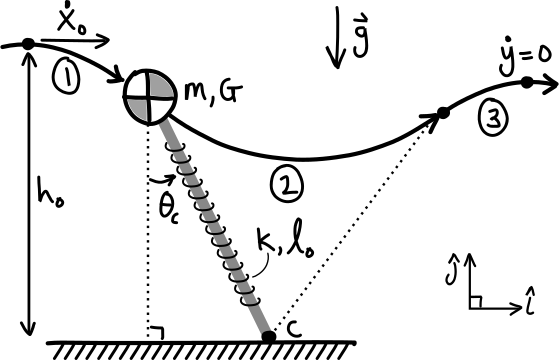
\includegraphics[width=0.7\textwidth]{Figures/SLIPSetup}\par
\end{centering}
\caption[Diagram: SLIP Model]{SLIP model. A point mass with mass $m$ at point $G$ is attached to a spring leg with spring constant $k$ and rest length $l_{0}$.  The gait starts when the position (x,y) of $G$  reaches the condition $\dot{y} = 0$. The subsequent motion is determined by the values for $\dot{x}_{0}$ and $h_{0}$. The leg makes contact with the ground at point $C$, and at contact is deflected from the vertical by an angle $\theta{c}$.}
\label{fig:SLIPSetup}
\end{figure}
%

The model is concerned with the stance portion of the gait cycle, which is defined in figure \ref{fig:SLIPGait} as the portion of the gait during which the leg is contacting the ground.  The initial conditions for a gait cycle are $\dot{x}_{0}$, the horizontal velocity, and $h_{0}$, the height of the locomotive, at the start of the gait cycle. The gait cycle starts at the point or moment at which $\dot{y}(x,t) = \dot{y}_{0}(x) = 0$. The angle that the leg makes with a vertical at the time of contact is $\theta_c$. The initial contact angle $\theta_c$ is the most important parameter in this model. For now, assume that $\theta_c$ is reset to the same value at the start of each stance. Later, $\theta_c$ will be controlled in order to explore the stability of the model. Throughout the stance, point C does not slip.

% FIGURE
\begin{figure}[h]		% h="here" t="top" b="bottom" p="separate page"
\begin{centering}
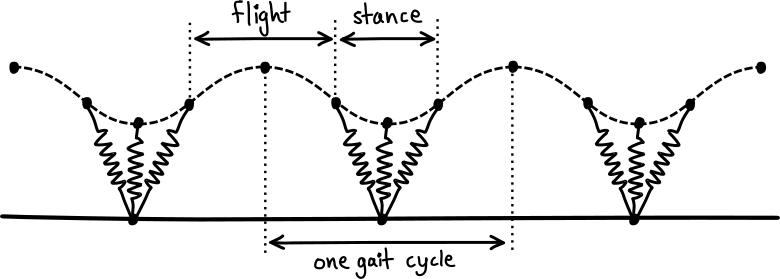
\includegraphics[width=0.9\textwidth]{Figures/SLIPGait}\par
\end{centering}
\caption[Diagram: SLIP Gait]{SLIP gait. The SLIP gait cycle can be divided into a flight, when the leg is not in contact with the ground, and a stance.}
\label{fig:SLIPGait}
\end{figure}
%

One way in which this model is distinct from the collisional model is that the contact of the locomotive with the ground is not impulsive. Additionally, it makes more sense to describe this model in terms of force interactions, rather than energy interactions as for the point mass and collisional models. The leg is modeled as a spring with spring constant $k$ and rest length $l_0$. As a result, the motion is also fully elastic, not quasi-elastic. This means that locomotion in this model is more efficient than in most cases of the collisional model since there is energy dissipation in the collisional model.

The gait cycle is divided into three portions, as denoted in figure \ref{fig:SLIPSetup}: (1) incoming flight, (2) stance, and (3) outgoing flight. The free body diagrams in figure \ref{fig:SLIPFBD} correspond to the three portions of the gait cycle. Linear momentum balance on the point mass yields

\begin{displaymath}
   m\vec{\mathbf{a}} = \left\{
     \begin{array}{ll}
        -mg \hat{\mathbf{j}} & : \mbox{flight, (1) and (3)} \\
       -mg \hat{\mathbf{j}} + \hat{\mathbf{F}}_s & : \mbox{stance, (2)} \\
     \end{array}
   \right.
\end{displaymath}

where $\hat{\mathbf{F}}_s$ is given by Hooke's Law,

\begin{equation}
\vec{\mathbf{F}}_s = k (l_0 - |\vec{\mathbf{r}}_{G/C}| ) \frac{\vec{\mathbf{r}}_{G/C}}{|\vec{\mathbf{r}}_{G/C}|}
\end{equation}

% FIGURE
\begin{figure}[h]		% h="here" t="top" b="bottom" p="separate page"
\begin{centering}
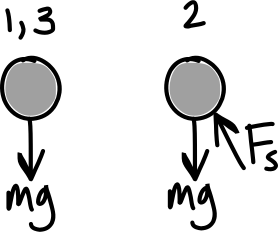
\includegraphics[width=0.2\textwidth]{Figures/SLIPFBD}\par
\end{centering}
\caption[Diagram: Free Body Diagrams for the SLIP Model]{Free body diagrams for the SLIP model. The locomotive in the SLIP model is a point mass. The left free body diagram corresponds to flight (labeled 1 and 3 in figure \ref{fig:SLIPSetup}) and the right free body diagram corresponds to stance. In stance, the force conveyed through the leg $F_{s}$ changes direction, unlike in the collisional model.}
\label{fig:SLIPFBD}
\end{figure}
%

The outgoing flight begins when the length of the leg returns to its rest length. During the flight, the locomotive follows a parabolic trajectory. This is similar the brachiation\index{brachiation} discussed in section \ref{sec:TheCollisionalModel}.

Although figure \ref{fig:SLIPGait} in this section seems to indicate that the SLIP motion is perfectly periodic, the motion over several gaits is not necessarily so. The motion is only periodic if $\dot{x}(t)$ and $h(t)$ take on the initial values $\dot{x}_{0}$ and $h_{0}$ at the end of the first gait cycle when $\dot{y}(t) = 0$. A periodic gait cycle means that the motion is stable. Logically, it is the stable case that is interesting, The stable motion is characterized by appropriate choices for $\dot{x}_0$ and $h_0$, depending on the other parameters of the model. The SLIP model can portray both walking and running depending on how $\dot{x}_0$ and $h_0$ are chosen. Both modes of locomotion can be stable.


[chris: if we want to talk about actual numbers for metabolic cost, see Ruina's simplest walker paper]
